%\documentclass[../main.tex]{subfiles}


\begin{song}{title=\centering Knockin' On Heaven's Door \\\normalsize Bob Dylan  \vspace*{-0.3cm}}  %% sem se napíše jméno songu a autor
\moveright 4.5cm \vbox{      %Varianta č. 1  ---> Jeden sloupec zarovnaný na střed

\sloka
 ^{G}Mama, ^{D}take this badge off of me ^{Ami} 
 
 ^{G}I can't ^{D}use it ^{C}anymore. 
 
It's gettin' dark, too dark for me to see 

I feel like I'm knockin' on heaven's door.

\refren
^{G}Knock, knock, ^{D}knockin' on heaven's  ^{Ami}door.

^{G}Knock, knock, ^{D}knockin' on heaven's  ^{C}door. 
 
Knock, knock, knockin' on heaven's door.

Knock, knock, knockin' on heaven's door.

\sloka
Mama, put my guns in the ground 

I can't shoot them anymore. 

That long black cloud is comin' down 

I feel like I'm knockin' on heaven's door. 

\refren

}
\setcounter{Slokočet}{0}
\end{song}
\begin{figure}[h]
\centering
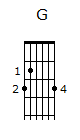
\includegraphics[scale=1.5]{../Akordy/g}
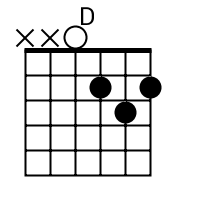
\includegraphics[scale=1.5]{../Akordy/d}
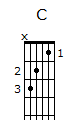
\includegraphics[scale=1.5]{../Akordy/c}
\includegraphics[scale=1.5]{../Akordy/Am}
\end{figure}
